%%%%%%%%%%%%%%%%%%%%%%%%%%%%%%%%%%%%%%%%%
% Fancyslides Presentation
% LaTeX Template
% Version 1.0 (30/6/13)
%
% This template has been downloaded from:
% http://www.LaTeXTemplates.com
%
% The Fancyslides class was created by:
% Paweł Łupkowski (pawel.lupkowski@gmail.com)
%
% License:
% CC BY-NC-SA 3.0 (http://creativecommons.org/licenses/by-nc-sa/3.0/)
%
%%%%%%%%%%%%%%%%%%%%%%%%%%%%%%%%%%%%%%%%%

%----------------------------------------------------------------------------------------
% PACKAGES AND OTHER DOCUMENT CONFIGURATIONS
%----------------------------------------------------------------------------------------

\documentclass{fancyslides}

\usepackage[utf8]{inputenc} % Allows the usage of non-english characters
\usepackage{times} % Use the Times font
\usepackage{booktabs} % Allows the use of \toprule, \midrule and \bottomrule in tables
\graphicspath{{images/}} % Location of the slide background and figure files

% Beamer options - do not change
\usetheme{default} 
\setbeamertemplate{navigation symbols}{} % Disable the slide navigation buttons on the bottom of each slide
\setbeamercolor{structure}{fg=\yourowntexcol} % Define the color of titles and fixed text elements (e.g. bullet points)
\setbeamercolor{normal text}{fg=\yourowntexcol} % Define the color of text in the presentation

%------------------------------------------------
% COLORS
% The following colors are predefined in this class: white, black, gray, blue, green and orange

% Define your own color as follows:
%\definecolor{pink}{rgb}{156,0,151}

\newcommand{\structureopacity}{0.75} % Opacity (transparency) for the structure elements (boxes and circles)

\newcommand{\strcolor}{blue} % Set the color of structure elements (boxes and circles)
\newcommand{\yourowntexcol}{white} % Set the text color

%----------------------------------------------------------------------------------------
% TITLE SLIDE
%----------------------------------------------------------------------------------------

%\newcommand{\titlephrase}{Make Pa} % Presentation title
%\newcommand{\name}{Sergio} % Presenter's name
%\newcommand{\affil}{} % Presenter's institution
%\newcommand{\email}{sergiogoro86@gmail.com} % Presenter's email address

\begin{document}

%\startingslide % This command inserts the title slide as the first slide

%----------------------------------------------------------------------------------------
%----------------------------------------------------------------------------------------
% PRESENTATION SLIDES
%----------------------------------------------------------------------------------------
%----------------------------------------------------------------------------------------

%------------------------------------------------
% Pointed
%------------------------------------------------

\fbckg{1.jpg} % Slide background image
\begin{frame}
\pointedsl{\$ Make Pa \ldots} % Text in this environment is printed in a circle and will be made large and uppercase - if you need to fit more text in you can reduce the font size within the \pointedsl{} bracket as usual, e.g. \pointedsl{\large smaller main point}
\end{frame}


%------------------------------------------------
% Framed
%------------------------------------------------

%\fbckg{2.jpg} % Slide background image
%\begin{frame}
%\framedsl{Qu\`e es el Pa?} % Text in this environment will be made large, uppercase and will wrap multiple lines
%\end{frame}

%------------------------------------------------
% Itemized
%------------------------------------------------

%\fbckg{2.jpg} % Slide background image
%\begin{frame}
%\itemized{ % This environment simply prints a series of bullet points
%\item Pa amb llevat
%\item Massa madre
%\item Pa de massa madre
%}
%\end{frame}

%------------------------------------------------
% \pitem
%------------------------------------------------

%\fbckg{2.jpg} % Slide background image
%\begin{frame}
%\framedsl{\pitem{Massa madre} \pitem{Pa amb massa madre} \fitem{Pa amb llevat ¿quimic?}} % Text in \pitem commands will be printed one after another on separate slides until all are displayed
%\end{frame}

%------------------------------------------------
% Enumerate
%------------------------------------------------

\fbckg{pa_fons.jpg} % Slide background image
\begin{frame}
\misc{ % Anything can be placed inside the \misc{} command
%\Huge
\$ \texttt{apropos Pa}\\
%\itemized{ 
%\item Pa amb llevat\\
%\item Pa amb massa mare natural\\
%}
Pa amb llevat\\
Pa amb massa mare natural\\
} %misc

%\ldots\\

\misc{
\$ \texttt{make Pa --llevat -n 2 -t Bagguete}\\
\footnotesize
Requires:\\
\small
$1/2$ Kg. Farina\\
325 g. H$_2$O\\
10 g. Sal\\
Llavors\\
2 g. Llevat sec(x3 fresc)
} %misc

%\itemized{ 
%\item 1/2 Kg. Farina\\
%\item 325 g. H$_2$O
%\item 2 g. Llevat sec (= 6g. llevat fresc)
%\item 10 g. Sal
%\item Llavors
%} %itemized



%\begin{enumerate}
%\centering
%\item Pa amb llevat
%\item Massa madre
%\item Pa de massa madre
%\end{enumerate}


\end{frame}


%------------------------------------------------
% Table
%------------------------------------------------

\fbckg{pa_fons.jpg} % Slide background image
\begin{frame}
\misc{ % Anything can be placed inside the \misc{} command


\$ \texttt{man Pa}\\

\begin{table}[h]
\begin{tabular}{l l l l}

\toprule
%\textbf{(1)Barrejar} & \textbf{(2)Amassar} & \textbf{(3)Nevera} & \textbf{(4)Fornejar}\\
\textbf{(1)Amassar} & \textbf{(2)Nevera} & \textbf{(3)Crear} & \textbf{(4)Fornejar}\\
\midrule

Empaquetar & Nevera $12\approx24$ h. & Sentir & Preescalfar 250ºC\\
Reposar 15\' &  & Airejar 1h. (opt) & Meter + $1/2$H$_2$O @ bandeja\\
Empquetar(2) &  & Estendre & Apagar 10m\\
Reposar 15\' &  & Tallar en 2 & Engegar 200º\\
Empquetar(3) &  & Humitejar & Fornejar $25\approx40$m\\
Reposar 15\' &  & Sembrar & \\
Empquetar(4) &  & Trenar & \\


\bottomrule
\end{tabular}
\end{table}
}
\end{frame}

%------------------------------------------------
% Image slide
%------------------------------------------------

\fbckg{2.jpg} % Slide background image
\begin{frame}
\misc{ % Anything can be placed inside the \misc{} command
Imatges de empaquetar
\begin{figure}[h]
\includegraphics[width=0.4\linewidth]{placeholder}
\end{figure}
}
\end{frame}


%------------------------------------------------
% Image slide
%------------------------------------------------

\fbckg{2.jpg} % Slide background image
\begin{frame}
\misc{ % Anything can be placed inside the \misc{} command
Imatges de crear
\begin{figure}[h]
\includegraphics[width=0.4\linewidth]{placeholder}
\end{figure}
}
\end{frame}


%------------------------------------------------
% Enumerate
%------------------------------------------------

%\fbckg{pa_fons.jpg} % Slide background image
%\begin{frame}
%\misc{ % Anything can be placed inside the \misc{} command
%\Large
%\$ \texttt{make Pa --llevat -n 2 -t Bagguete}\\
%Ingredients:
%\itemized{ 
%\item 1/2 Kg. Farina\\
%\item 325 g. H$_2$O
%\item 2 g. Llevat sec (= 6g. llevat fresc)
%\item 10 g. Sal
%\item Llavors
%}
%\begin{enumerate}
%\centering
%\item Pa amb llevat
%\item Massa madre
%\item Pa de massa madre
%\end{enumerate}
%} %misc
%\end{frame}


%------------------------------------------------
% Image slide
%------------------------------------------------

%\fbckg{2.jpg} % Slide background image
%\begin{frame}
%\misc{ % Anything can be placed inside the \misc{} command
%Figures can also be included with the \texttt{\textbackslash misc\{\}} command:
%\begin{figure}[h]
%\includegraphics[width=0.4\linewidth]{placeholder}
%\end{figure}
%}
%\end{frame}

%------------------------------------------------
% Thank you
%------------------------------------------------

\fbckg{mans_a_la_massa.jpg} % Slide background image
\begin{frame}
\thankyou % Inserts a thank you slide
\end{frame}

%------------------------------------------------
% Credits
%------------------------------------------------

%\fbckg{blank} % A blank background can be used instead of an image
%\begin{frame}
%\sources{ % An environment for giving credit for slide backgrounds, images will need to be scaled down if there are more than two
%\includegraphics[scale=0.048]{1.jpg} \ flickr/lovelornpoets\\
%\includegraphics[scale=0.048]{1.jpg} \ youtube/ibanyarza\\
%}
%\end{frame}

%------------------------------------------------
% Resources
%------------------------------------------------

\fbckg{2.jpg} % Slide background image
\begin{frame}
\misc{ % Anything can be placed inside the \misc{} command
Resources:
\begin{figure}[h]
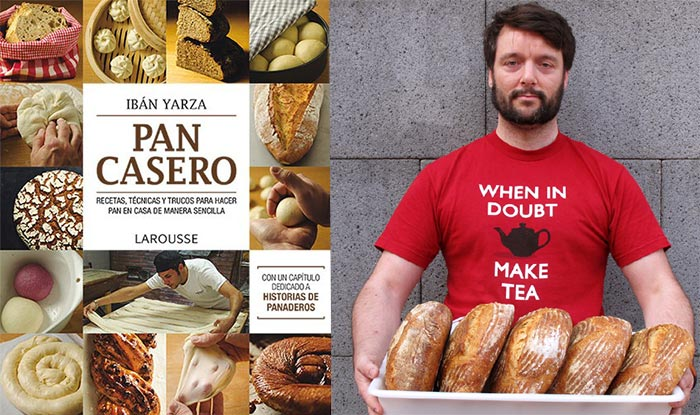
\includegraphics[width=0.4\linewidth]{Iban_pancasero}
\end{figure}
elforodelpan.com\\
lamemoriadelpan.com\\
tequedasacenar.com\\
}
\end{frame}

%------------------------------------------------
% Table
%------------------------------------------------

\fbckg{pa_fons.jpg} % Slide background image
\begin{frame}
\misc{ % Anything can be placed inside the \misc{} command
%Tables can be included with the \texttt{\textbackslash misc\{\}} command:
Trade-off
\begin{table}[h]
\begin{tabular}{l l l}
\toprule
\textbf{Pa amb \ldots} & \textbf{Llevat} & \textbf{Massa madre}\\
\midrule
time & Rapid & Lento \\
top & Senzill & Elaborat \\
stdout & Bonn\'issim & Suprem \\
\bottomrule
\end{tabular}
\end{table}
}
\end{frame}


%----------------------------------------------------------------------------------------

\end{document}
